\documentclass[12pt,letterpaper,twocolumn,openany,nodeprecatedcode,bg=none]{dndbook}
\usepackage[english]{babel}
\usepackage[utf8]{inputenc}
\usepackage{longtable,booktabs,array}
\usepackage{calc}
\usepackage{etoolbox}
\usepackage{caption}
\AtBeginEnvironment{longtable}{\small}

% Fix for Pandoc 3.1.7+ image handling
\providecommand{\pandocbounded}[1]{#1}

% Pandoc's compact list helper
\providecommand{\tightlist}{%
  \setlength{\itemsep}{0pt}\setlength{\parskip}{0pt}}

% Remove "Figure N:" prefix from captions
\captionsetup{labelformat=empty}

% Remove section numbering
\setcounter{secnumdepth}{0}

\begin{document}

\title{Necromancer}
\author{Class Handbook}
\date{}
\maketitle

\onecolumn

\emph{Your trusty class handbook for the Old Scrolls roleplaying game.}

\clearpage

\begin{figure}
\centering
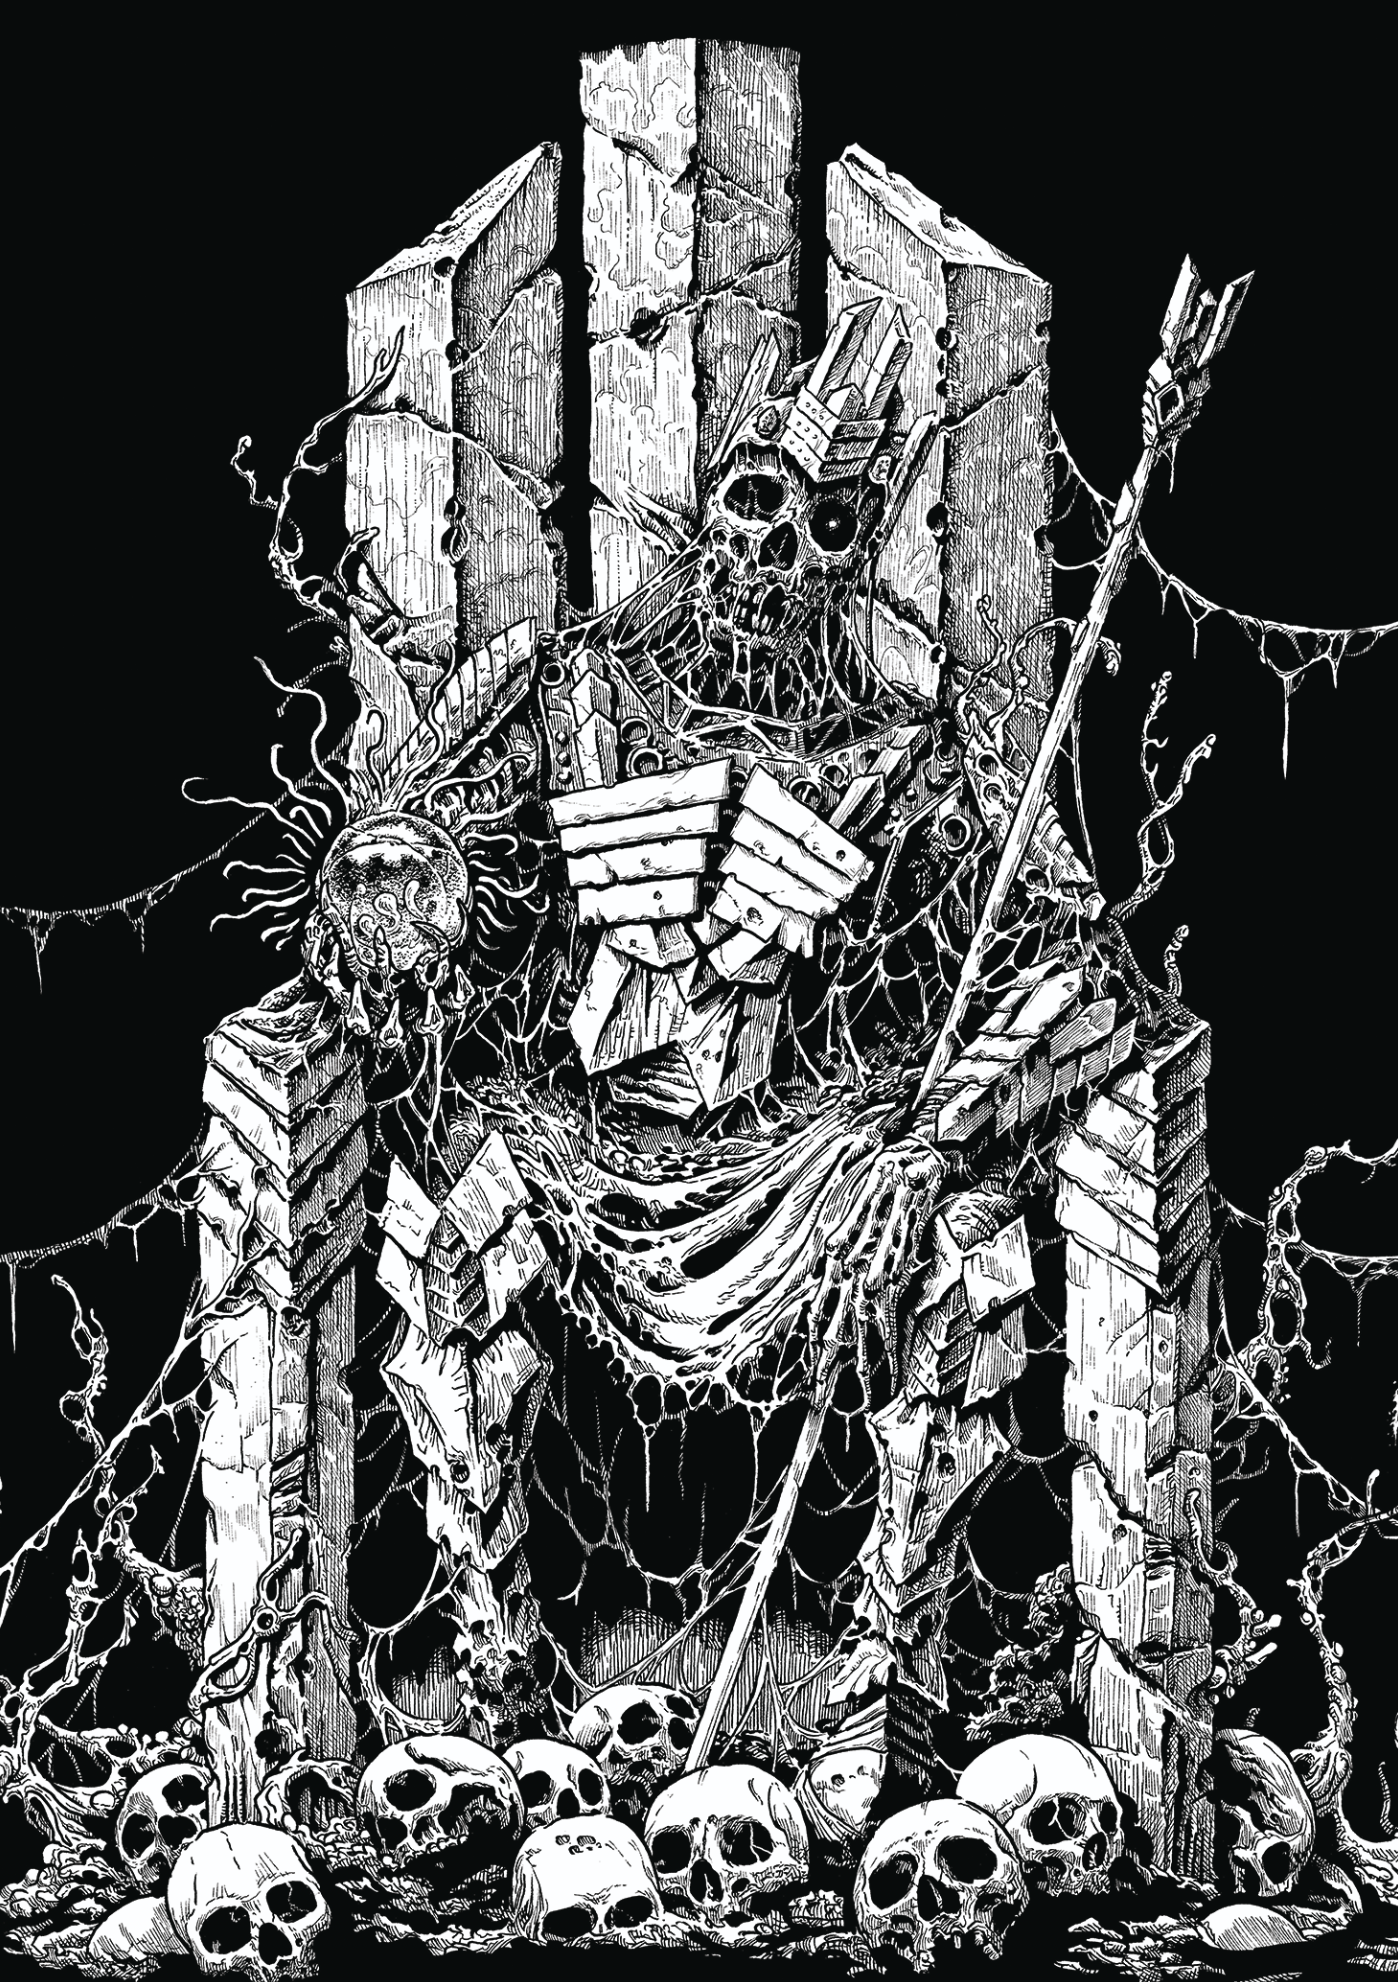
\includegraphics[width=1\linewidth,height=\textheight,keepaspectratio]{lich.png}
\caption{\emph{A necromancer seeks domination over death itself}}
\end{figure}

\clearpage

\section{Necromancer}\label{necromancer}

Necromancers are often foul, evil magic users who have ignored the
cautionary tales of the dangers of death magic and have sought out the
ancient profane rituals of necromancy. The ultimate goal of most
necromancers is the mastery over death itself, ascendency to eternal
undeath and lichdom as the master of their own personal army of mindless
servants.

\subsection{Core Necromancer Traits}\label{core-necromancer-traits}

\begin{longtable}[]{@{}
  >{\raggedright\arraybackslash}p{(\linewidth - 2\tabcolsep) * \real{0.2542}}
  >{\raggedright\arraybackslash}p{(\linewidth - 2\tabcolsep) * \real{0.7458}}@{}}
\toprule\noalign{}
\begin{minipage}[b]{\linewidth}\raggedright
\textbf{Primary Ability}
\end{minipage} & \begin{minipage}[b]{\linewidth}\raggedright
Intelligence
\end{minipage} \\
\midrule\noalign{}
\endhead
\bottomrule\noalign{}
\endlastfoot
\textbf{Hit Points} & 8 at 1st level, 6 per level gained after 1st \\
\textbf{Saving Throw Proficiencies} & Intelligence, Wisdom \\
\textbf{Skill Proficiencies} & Choose any 2 skills. If you choose a
skill you already have, you gain expertise with it. \\
\textbf{Weapon Proficiencies} & Choose 1: Blade, Blunt, Bow, Mechanical,
Polearm, and Shield \\
\textbf{Starting Equipment} & Padded Jacket, Grimoire, Robe, Dagger \\
\end{longtable}

\subsection{Necromancer Features
Table}\label{necromancer-features-table}

\begin{longtable}[]{@{}
  >{\raggedright\arraybackslash}p{(\linewidth - 6\tabcolsep) * \real{0.0794}}
  >{\raggedright\arraybackslash}p{(\linewidth - 6\tabcolsep) * \real{0.1746}}
  >{\raggedright\arraybackslash}p{(\linewidth - 6\tabcolsep) * \real{0.1111}}
  >{\raggedright\arraybackslash}p{(\linewidth - 6\tabcolsep) * \real{0.6349}}@{}}
\toprule\noalign{}
\begin{minipage}[b]{\linewidth}\raggedright
Level
\end{minipage} & \begin{minipage}[b]{\linewidth}\raggedright
Proficiency
\end{minipage} & \begin{minipage}[b]{\linewidth}\raggedright
Rituals
\end{minipage} & \begin{minipage}[b]{\linewidth}\raggedright
Class Features
\end{minipage} \\
\midrule\noalign{}
\endhead
\bottomrule\noalign{}
\endlastfoot
1 & +2 & 1 & Master of Life and Death, Tools of Death \\
2 & +2 & 2 & Soul Sight, Bonus Ritual \\
3 & +2 & 2 & Death's Harvest, Tool of Death \\
4 & +2 & 3 & Ability Score Improvement, Bonus Ritual \\
5 & +3 & 3 & Endless Rituals \\
6 & +3 & 4 & Bonus Ritual \\
7 & +3 & 4 & Tool of Death, Unholy Vigor \\
8 & +3 & 5 & Ability Score Improvement, Bonus Ritual \\
9 & +4 & 5 & Unholy Endurance \\
10 & +4 & 6 & Bonus Ritual, Greater Heresy \\
\end{longtable}

\twocolumn

\subsection{Necromancer Features}\label{necromancer-features}

As a necromancer, you gain the following class features when you reach
the specified levels. These features are listed on the Necromancer
Features table.

\subsection{Level 1: Master of Life and
Death}\label{level-1-master-of-life-and-death}

As a necromancer, you have learned to breach the barrier between life
and death. You command the dead, allowing you to draw ancient spirits to
serve you. These spirits animate corpses that your magic alters and
strengthens.

\textbf{Saving Throws.} The saving throw DC of your necromancer features
is 8 + your Intelligence modifier + your proficiency bonus.

\textbf{Rituals.} As a necromancer, you can call upon unquiet souls to
do your bidding. You master blasphemous rituals, forbidden magics that
allow you to animate the dead or call forth spirits from their slumber
to serve you. You start with one ritual and learn more as you gain
levels. When you gain a level, you can replace a ritual you know with a
new one. Each ritual has a level. Your level must be greater than or
equal to its level for you to take it.

\textbf{Controlling the Dead.} Each summoned undead creature provides a
stat block, including the initiative it acts on. Undead do not roll
initiative, they have static initiative. When you summon an undead
creature, it appears within 30 feet of you. You decide their course of
action, issuing a general command that they continue to fulfill. The
undead can fulfill any task you wish, but lack specialized knowledge.
You could not leave them in a forge and command them to make a sword,
but they could assist by carrying water buckets, stocking a fire, and
working the forge under your supervision. They lack the creative spark
to create new things or work autonomously.

\textbf{Soul Focus.} When you use a ritual to create undead, it requires
your soul focus. The next time you use another ritual, the one that
needed your soul focus ends.

\subsection{Level 1: Tools of Death}\label{level-1-tools-of-death}

Your ability to pierce the veil between life and death allows you to
craft objects infused with death energy. You gain two tools of death
from among those listed at the end of this class.

\textbf{Dark Arts.} Many of your tools require an action to use. If you
use your action to use a ritual, you can also use a tool that turn
without using an additional action.

\subsection{Level 2: Bonus Ritual}\label{level-2-bonus-ritual}

You gain an additional ritual.

\subsection{Level 2: Soul Sight}\label{level-2-soul-sight}

As a magic action, you can perceive the flow of life and death around
you. You can detect the presence of living and undead creatures within
60 feet. You do not learn their exact location, but you learn their
number. This sight extends through physical barriers.

\subsection{Level 3: Death's Harvest}\label{level-3-deaths-harvest}

Once per turn when a creature within 30 feet of you dies, you regain hit
points equal to your Intelligence modifier.

\subsection{Level 3: Tool of Death}\label{level-3-tool-of-death}

You gain an additional tool of death.

\subsection{Level 4: Ability Score
Improvement}\label{level-4-ability-score-improvement}

You gain a +1 bonus to two abilities of your choice.

\subsection{Level 4: Bonus Ritual}\label{level-4-bonus-ritual}

You gain an additional ritual.

\subsection{Level 5: Endless Rituals}\label{level-5-endless-rituals}

At the start of your turn, any undead created by your currently active
ritual that are destroyed return to unlife with full hit points.

\subsection{Level 6: Bonus Ritual}\label{level-6-bonus-ritual}

You gain an additional ritual.

\subsection{Level 7: Tool of Death}\label{level-7-tool-of-death}

You gain an additional tool of death.

\subsection{Level 7: Unholy Vigor}\label{level-7-unholy-vigor}

On your turn, you can gain a failed death save to grant all undead
created by your rituals an extra action on their next turn.

\subsection{Level 8: Ability Score
Improvement}\label{level-8-ability-score-improvement}

You gain a +1 bonus to two abilities of your choice.

\subsection{Level 8: Bonus Ritual}\label{level-8-bonus-ritual}

You gain an additional ritual.

\subsection{Level 9: Unholy Endurance}\label{level-9-unholy-endurance}

The first time you take damage while at 0 hit points each turn, roll a
d20. On a 10 or higher, you do not take that damage and ignore all
damage you would take for the rest of the turn.

\subsection{Level 10: Bonus Ritual}\label{level-10-bonus-ritual}

You gain an additional ritual.

\subsection{Level 10: Greater Heresy}\label{level-10-greater-heresy}

You can now cast two rituals that require your soul focus, or you can
use the same one twice to double the number of undead you can create.

\clearpage

\section{Rituals}\label{rituals}

Rituals that require your soul focus note that in their duration entry.

\subsection{Animate Mummy}\label{animate-mummy}

\textbf{Level 6 Ritual (Necromancer)}

\textbf{Casting Time:} 1 action

\textbf{Range:} 30 feet

\textbf{Duration:} Permanent (Soul Focus)

You send a call deep into the realm of the dead to awaken the ancient,
slumbering spirit of a long dead hero. The spirit manifests as a mummy
that uses the stats below.

\textbf{Animated Mummy}

\begin{itemize}
\tightlist
\item
  \textbf{AC} 15
\item
  \textbf{HP} 9 per necromancer level
\item
  \textbf{Tests} +3 (Str +7)
\item
  \textbf{Fearsome Presence.} Creatures attacked by the mummy are goaded
  by it for one round.
\item
  \textbf{Initiative 5: Brutal Slams}

  \begin{itemize}
  \tightlist
  \item
    Two melee attacks
  \item
    Attack bonus equal to your proficiency + your Intelligence modifier
  \item
    2d10 bludgeoning damage
  \end{itemize}
\end{itemize}

\subsection{Animate Skeletons}\label{animate-skeletons}

\textbf{Level 2 Ritual (Necromancer)}

\textbf{Casting Time:} 1 action

\textbf{Range:} 30 feet

\textbf{Duration:} Permanent (Soul Focus)

You conjure forth the spirits of slain warriors to animate skeletons of
up to size Medium. Each skeleton has stats listed below. The number of
skeletons you can animate depends on your level. If you invoke this
ritual and already have skeletons animated with it, you animate
additional ones until you reach your limit. You animate one skeleton at
level 1, two at level 3, three at level 5, four at level 7, and five at
level 9.

\textbf{Animated Skeleton}

\begin{itemize}
\tightlist
\item
  \textbf{AC} 16
\item
  \textbf{HP} 8
\item
  \textbf{Tests} +0 (Dex +2)
\item
  \textbf{Death Splinters.} If killed by a melee attack, the creature
  that destroyed it takes 1d8 piercing damage.
\item
  \textbf{Initiative 20: Slashing Claws}

  \begin{itemize}
  \tightlist
  \item
    One melee attack
  \item
    Attack bonus equal to your proficiency + your Intelligence modifier
  \item
    1d6 slashing damage
  \end{itemize}
\end{itemize}

\subsection{Animate Zombies}\label{animate-zombies}

\textbf{Level 1 Ritual (Necromancer)}

\textbf{Casting Time:} 1 action

\textbf{Range:} 30 feet

\textbf{Duration:} Permanent (Soul Focus)

You call forth spirits of the dead to animate nearby corpses that are up
to size Medium. Each zombie has stats listed below. The number of
corpses you can animate depends on your level. If you invoke this ritual
and already have zombies animated with it, you animate additional ones
until you reach your limit. You animate one zombie at level 1, two at
level 3, three at level 5, four at level 7, and five at level 9.

\textbf{Animated Zombie}

\begin{itemize}
\tightlist
\item
  \textbf{AC} 12
\item
  \textbf{HP} 12
\item
  \textbf{Tests} +0 (Str, Con +2)
\item
  \textbf{Death Proof (15+).} When reduced to 0 hit points by damage
  other than radiant, roll a d20. On 15+ this creature is instead
  reduced to 1 hit point.
\item
  \textbf{Initiative 5: Rend and Tear}

  \begin{itemize}
  \tightlist
  \item
    One melee attack
  \item
    Attack bonus equal to your proficiency + your Intelligence modifier
  \item
    1d8 bludgeoning damage
  \end{itemize}
\end{itemize}

\clearpage

\subsection{Call Death Knight}\label{call-death-knight}

\textbf{Level 10 Ritual (Necromancer)}

\textbf{Casting Time:} 1 action

\textbf{Range:} 30 feet

\textbf{Duration:} Permanent (Soul Focus)

You send a call deep into the realm of the dead to awaken the ancient,
slumbering spirit of a long dead hero. The spirit manifests as a death
knight that uses the stats below.

\textbf{Death Knight}

\begin{itemize}
\tightlist
\item
  \textbf{AC} 18
\item
  \textbf{HP} 9 per necromancer level
\item
  \textbf{Tests} +4 (Str, Con, Wis +8)
\item
  \textbf{Doom Reaper.} Can move through but cannot end a turn inside a
  solid object.
\item
  \textbf{Initiative 15: Doom Blade}

  \begin{itemize}
  \tightlist
  \item
    Three melee attacks
  \item
    Attack bonus equal to your proficiency + your Intelligence modifier
  \item
    2d10 slashing damage
  \end{itemize}
\item
  \textbf{Initiative 15: Unholy Fire}

  \begin{itemize}
  \tightlist
  \item
    Target point within 120 feet
  \item
    Creatures within 20 feet of that point are affected
  \item
    Dexterity save using necromancer's save DC
  \item
    Failure: 6d6 fire damage
  \item
    Success: Half damage
  \end{itemize}
\end{itemize}

\subsection{Call Wraith}\label{call-wraith}

\textbf{Level 8 Ritual (Necromancer)}

\textbf{Casting Time:} 1 action

\textbf{Range:} 30 feet

\textbf{Duration:} Permanent (Soul Focus)

You draw forth a hateful spirit into this realm. The spirit manifests as
a wraith that uses the stats below.

\textbf{Wraith}

\begin{itemize}
\tightlist
\item
  \textbf{AC} 13
\item
  \textbf{HP} 7 per necromancer level
\item
  \textbf{Tests} +3 (Wis, Cha +6)
\item
  \textbf{Incorporeal.} Can move through but cannot end a turn inside a
  solid object.
\item
  \textbf{Insubstantial (16+).} The first time this creature takes
  damage on a turn, roll a d20. On a 16 or higher, this creature takes
  no damage that turn.
\item
  \textbf{Fly.} This creature can fly.
\item
  \textbf{Initiative 15: Life Drain}

  \begin{itemize}
  \tightlist
  \item
    One melee attack
  \item
    Attack bonus equal to your proficiency + your Intelligence modifier
  \item
    2d10 necrotic damage, and a creature within 30 feet may regain 2d10
    hit points
  \end{itemize}
\end{itemize}

\subsection{Call Wrathful Ghost}\label{call-wrathful-ghost}

\textbf{Level 4 Ritual (Necromancer)}

\textbf{Casting Time:} 1 action

\textbf{Range:} 30 feet

\textbf{Duration:} Permanent (Soul Focus)

You draw the ghost of someone who died a painful death. The spirit
manifests using the stats below.

\textbf{Wrathful Ghost}

\begin{itemize}
\tightlist
\item
  \textbf{AC} 13
\item
  \textbf{HP} 5 per necromancer level
\item
  \textbf{Tests} +1 (Cha +4)
\item
  \textbf{Incorporeal.} Can move through but cannot end a turn inside a
  solid object.
\item
  \textbf{Insubstantial (16+).} The first time this creature takes
  damage on a turn, roll a d20. On a 16 or higher, this creature takes
  no damage that turn.
\item
  \textbf{Fly.} This creature can fly.
\item
  \textbf{Initiative 10: Frightening Howl}

  \begin{itemize}
  \tightlist
  \item
    Hostile creatures in melee range must make saves
  \item
    Wisdom save using necromancer's save DC
  \item
    Failure: 1d4 psychic damage per 2 levels and frightened of the ghost
    for 1 round
  \item
    Success: Half damage
  \end{itemize}
\end{itemize}

\subsection{Curse of Death's Doorstep}\label{curse-of-deaths-doorstep}

\textbf{Level 6 Ritual (Necromancer)}

\textbf{Casting Time:} 1 action

\textbf{Range:} 120 feet

\textbf{Target:} 1 creature

\textbf{Duration:} 3 rounds

You weave necromantic energy through a creature's spirit, sending
tendrils into the future to draw its death hurtling toward it. The
target creature gains a death curse, its life energy bleeding away each
time death comes to call. Once per round when a creature within 30 feet
of it dies, it takes 3d12 necrotic damage, or 4d10 at level 8.

\subsection{Gaze of the Bloody Skull}\label{gaze-of-the-bloody-skull}

\textbf{Level 4 Ritual (Necromancer)}

\textbf{Casting Time:} 1 action

\textbf{Range:} 30 feet

\textbf{Duration:} 1 round

The skin covering your skull peels back, revealing a horrid, bloody mask
that leaves creatures shrieking in terror. Creatures of your choice
within 30 feet of you must make Wisdom saves. On a failed save, a
creature is frightened of you and cannot move closer to you.

\subsection{Vampiric Harvest}\label{vampiric-harvest}

\textbf{Level 1 Ritual (Necromancer)}

\textbf{Casting Time:} 1 action

\textbf{Range:} 120 feet

\textbf{Target:} 1 creature

\textbf{Duration:} 1 round

You infuse an aura of death energy around a creature, allowing you to
collect its life energy and share it with an ally.

Once per turn when the target takes damage, you gain one blood point. At
the start of your next turn when this spell's duration expires, a
creature of your choice within range regains 3 hit points per blood
point you collected. You then lose all blood points.

\clearpage

\section{Tools of Death}\label{tools-of-death}

If you lose a tool, you can craft another one as part of a long rest.
The item is ready when the long rest ends. You can replace one tool for
each long rest.

\subsection{Death Mask}\label{death-mask}

You weave a ghoulish mask from skin taken from an embalmed corpse. When
you wear the mask you gain the following benefits.

When making Charisma checks to influence undead creatures, add your
Intelligence modifier as a bonus to the roll.

As a magic attack action, you can stare at a creature within 120 feet
and fill it with dread. It must make a Wisdom save. On a failed save, it
is frightened of you for one round and takes psychic damage based on
your level.

The damage is 1d4 at level 1, 2d4 at level 3, 3d4 at level 5, and 4d4 at
level 8.

\subsection{Death-Eyed Skull}\label{death-eyed-skull}

You collect a skull and scribe it with blasphemous runes of death and
annihilation. You can present the skull and channel power through it,
causing a sickly beam of crimson energy to emit from it as a magic
attack action. This is an attack against one target with a range of 120
feet that uses your Intelligence modifier on its attack and damage
rolls. On a hit, the target comes under a death curse and suffers
psychic damage based on your level. While cursed, undead creatures have
advantage on attacks against it for one round.

The damage is 1d4 at level 1, 2d4 at level 3, 3d4 at level 5, and 4d4 at
level 8.

\subsection{Emissary Skull}\label{emissary-skull}

You have the skull of a linguist and ambassador. Treated with runes, it
retains a shadow of its former knowledge.

If the skull is daubed with blood or other remains taken from a slain
creature, it gains the knowledge of all languages that creature speaks.
You can speak, understand, and read those languages while you hold the
skull. If you use this ability again, the skull loses the prior
languages it learned, replacing them with the new ones.

\subsection{Scythe of Reaping}\label{scythe-of-reaping}

You imbue a scythe with the energies that simmer between life and death.
It becomes a cutting tool that you can use to reap life energy from your
enemies. The scythe is a two-handed, reach melee weapon that does 1d6
slashing damage.

In your hands, the weapon uses your Intelligence modifier for its attack
and damage bonus.

At higher levels, you gain reaper dice as the scythe's cuts open the
gate between life and death. Your reaper dice are 1d6 at level 3, 3d6 at
level 5, and 4d6 at level 8.

When you hit a hostile creature with the scythe, you can roll the reaper
dice and apply the total as necrotic damage to the target of your attack
or as healing to a creature within melee range of you.

\subsection{Thief's Hands}\label{thiefs-hands}

You have acquired the severed hands of a dead thief and, with your
magic, have imbued the thief's cunning into them.

The hands are two Tiny objects with AC 15, 2 hit points each, and a test
bonus equal to your Intelligence modifier + your proficiency bonus. They
have advantage on all Stealth checks. They have a climb speed.

As a magic action, you can direct them to open doors, search through
treasure piles, and take other actions as you direct. As a search
action, you can project your senses through one of them, allowing you to
see and hear everything it senses for one round.

The hands understand how to use lock picks and can be directed to pick
locks and disable traps if they are carrying the appropriate tools.

\onecolumn

\begin{figure}
\centering
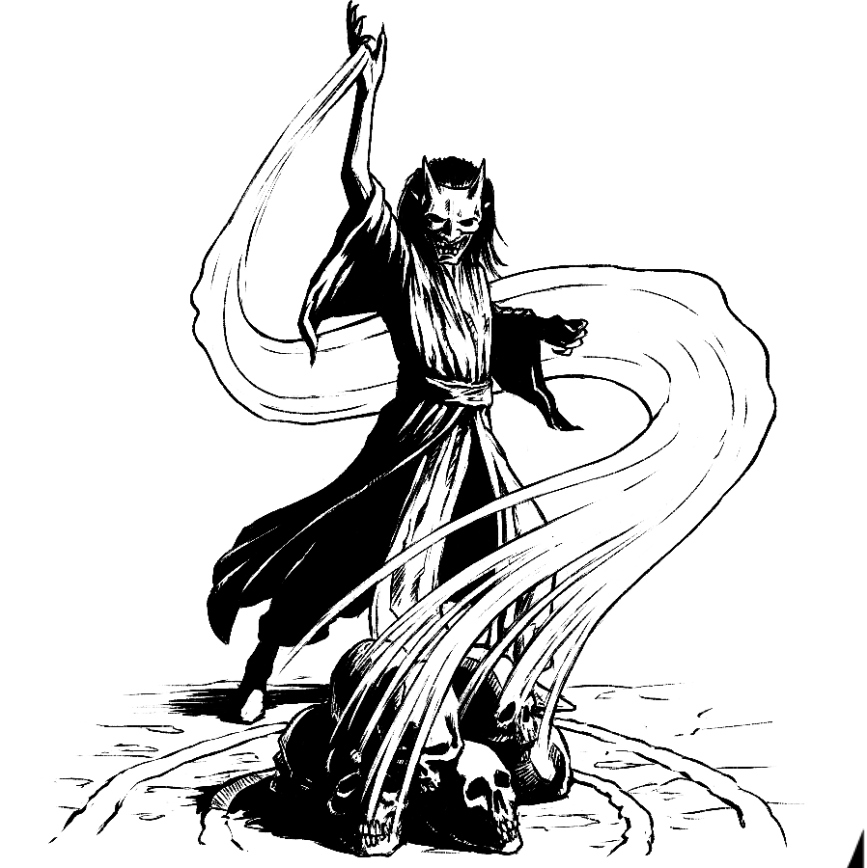
\includegraphics[width=0.9\linewidth,height=\textheight,keepaspectratio]{necromancer.png}
\caption{\emph{The powers of necromancy are quite useful in the right
hands}}
\end{figure}

\end{document}